\documentclass{hw}
\usepackage[version=3]{mhchem}
\usepackage{nuc}
\usepackage{graphicx}
\graphicspath{ {images/}}

\author{J.R. Powers-Luhn}
\date{2016/09/01}
\title{Homework \#1}

\begin{document}

\problem{2-1}
	What target isotope must be used for forming the compound nucleus $ \ce{^{24}_{11}Na} $ when the incident projectile is:
	\begin{enumerate}
		\item a neutron
		\item a proton
		\item an alpha particle?
	\end{enumerate}
\solution
	\part A neutron will increase the mass number, $ A $, by one, but leave the element number, $ Z $, unchanged. Therefore, the answer is a lighter isotope of Neon: \ce{^{23}_{11}Na}
	\part Capturing a proton increases both the mass number and element number by one: \ce{^{23}_{10}Ne}
	\part Capturing an $ \alpha $ particle increases the mass number by four and the element number by two: \ce{^{20}_{8}O}

\problem{2-4}
	A fission product of very considerable importance in thermal reactor operation is $ \ce{^{135}Xe}$, which has an enormous thermal absorption cross section of $ 2*10^6 b $. This nuclide can be produced either directly as a fission product or by beta decay of $ \ce{^{135}I} $, as indicated by the radioactive chains below:
%	\begin{rxn}
%		\ce{^{135}I} \arrow \ce{^{135}Xe}
%	\end{rxn}
	
	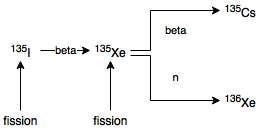
\includegraphics{470-1-2}
	
	Write the rate equations describing the concentration of $ \ce{^{135}I} $ and $ \ce{^{135}Xe} $ in a nuclear reactor. Then assuming a constant production rate of these isotopes from fission and transmutation rate by neutron capture, determine the steady-state or saturated concentration of $ \ce{^{135}Xe} $.
\solution
	$\ce{^{135}I}$ has one production path (production as a fission daughter) and one decay path ($\beta$ decay into $\ce{^{135}I}$). The rate equation is:
	\[ \dot{N}_{\ce{^{135}I}} = \phi\Sigma_{fission}\gamma_{\ce{^{135}I}}-\lambda_{\ce{^{135}I}}N_{\ce{^{135}I}} \]

	$\ce{^{135}Xe}$ is also produced by fission, as well as by the $\beta$ decay of $\ce{^{135}I}$. It is removed by $\beta$ decay as well as by neutron absorption:
	\[ \dot{N}_{\ce{^{135}Xe}} = \phi\Sigma_{fission}\gamma_{\ce{^{135}Xe}}+\lambda_{\ce{^{135}I}}N_{\ce{^{135}I}}-\lambda_{\ce{^{135}Xe}}N_{\ce{^{135}Xe}}-\sigma_{a} \phi N_{\ce{^{135}Xe}} \]

	In steady state, set $ \dot{N} = 0 $:

	Iodine:

	\begin{align*}
		\dot{N}_{\I{135}} &= 0 \rightarrow \\ 
		\lambda_I N_I &= \phi \Sigma_f \gamma_I \\
		N_{\I{135}} &= \frac{\phi \Sigma_f \gamma_I}{\lambda_I}
	\end{align*}

	Xenon:

	\begin{align*}
		\dot{N}_{Xe} &= 0 \rightarrow \\ 
		N_{Xe} \left( \lambda_{Xe} + \sigma_{Xe} \phi \right)&= \phi \Sigma_f \gamma_{Xe} + \lambda_I N_I  \\
		N_{Xe} &= \frac{\phi \Sigma_f \gamma_{Xe} + \lambda_I N_I}{\lambda{Xe} + \sigma_{Xe} \phi} \\
		&= \frac{\phi \Sigma_f \gamma_{Xe} + \phi \Sigma_f \gamma_I}{\lambda_{Xe} + \sigma_{Xe} \phi} \\
		N_{\Xe{135}} &= \frac{\phi \Sigma_f \left( \gamma_{Xe} + \gamma_I \right)}{\lambda_{Xe} + \sigma_{Xe} \phi}
	\end{align*}

\problem{2-6}
	Boron is a common material used to shield against thermal neutrons. Estimate the thickness of boron required to attenuate an incident thermal neutron beam to 0.1\% of its intensity. (Use the thermal cross section data in Appendix A.)
\solution
	From \textit{Duderstadt} Appendix A, $ \Sigma_t = 104cm^{-1}$ for Boron.
	
	\begin{align*}
		\left(\frac{1}{e}\right)^n &= \frac{1}{1000} \\
		e^{-n} &= 1000^{-1} \\
		e^n &= 1000 \\
		n &= ln(1000) \\
		\intertext{Dividing this by the macroscopic cross section $ \Sigma_t $ gives:}
		\frac{n}{\Sigma_t} &= \frac{ln(1000)}{\Sigma_t} \\
		&= 0.0664 cm
	\end{align*}

\problem{2-8}
	A free neutron is unstable against beta decay with a half-life of 11.7m. Determine the relative probability that a neutron will undergo beta-decay before being absorbed in an infinite medium. Estimate this probability for a thermal neutron in $ \ce{H_{2}O} $.
\solution
	We know that:
	\begin{align*}
		P_{absorption}\left(x\right) &= \Sigma_a\int_0^x e^{-\Sigma_a x}dx \\
		&= \sigma_a N \int_0^x e^{-\sigma_a x}dx
		\intertext{Assume that the incident particle is a thermal neutron with speed \text{$ \dot{x}=2.2*10^5cm/s $}. In this case, the neutron should travel a distance of $ \dot{x}\lambda $ before decaying:}
		&= \sigma_a N \int_0^{\dot{x}\lambda} e^{-\sigma_a x}dx \\
		&= 1-e^{-\sigma_a N \dot{x} \lambda}
		\intertext{The probability of decaying instead of being absorbed (assuming that these are the only two interaction modes:}
		1 &= P_{absorption} + P_{decay} \\
		P_{decay} &= 1-P_{absorption} \\
		&= e^{-\sigma_a N \dot{x} \lambda}
		\intertext{Substituting our speed \text{$ \dot{x}=2.2*10^5cm/s $}, half life $ \lambda=11.7m=702s $, and $ \sigma_a N=0.022 $ for a thermal neutron in $ H_{2} $O:}
		&= 2.11*10^{-1475594}
	\end{align*}
	
	To any reasonable approximation this may be treated as equal to zero.

\problem{2-10}
	How many mean free paths thick must a shield be designed in order to attenuate an incident neutron beam by a factor of 1000?
\solution
	We know that for every mean free path, $ \Sigma $, travelled, the incident beam attenuates by a factor of $ \frac{1}{e} $. Therefore:
	
	\begin{align*}
		\left(\frac{1}{e}\right)^n &= \frac{1}{1000} \\
		e^{-n} &= 1000^{-1} \\
		e^n &= 1000 \\
		n &= ln(1000) \\
		&= 6.91
	\end{align*}

\end{document}
